% Appendix: details of the replication (Section 1).  Requires \appendix before inclusion.
\section{Replication details}
\label{app:repl}

All numbers here are produced by \texttt{notebooks/01\_replication.ipynb} and guarded by the
tests in \texttt{tests/}. Notation: spending $t$ units of currency on an item buys the proportion
$Q(t)=\int_0^t\frac{ds}{as+b}=\frac1a\ln\!\big(1+\tfrac{at}{b}\big)$ of it, with $b=a/(e^a-1)$ so that $Q(1)=1$.

\subsection{The paper's Theorem~2: the competitive ratio of LIP(2)}

\emph{Reminder.} $\alpha(a)=\min_{1\ge x\ge y\ge0}S(x,y)/(x+1-y)$; the paper brackets it on a
uniform grid of step $1/N$ (exact ratio at grid points from above, worst cell corner of each term
of $S$ from below, using the monotonicity of $p_1,p_2$).

We implemented exactly this bracket and found that a uniform grid reproduces the stated numbers
only slowly: the upper bound is $0.82818$ at $N=50$ and $0.82815$ from $N=100$ on, but the lower
bound reaches $0.828$ only for $N\gtrsim2\cdot10^4$, i.e.\ $\sim4\cdot10^8$ cells. We therefore
added \emph{adaptive refinement}: starting from a $64\times64$ grid, a cell is split into four
only while its lower bound is below the best exact value found so far minus a tolerance. Since
every point of the triangle always lies in some leaf cell, the minimum of the leaf lower bounds
is a valid bound over the whole domain, exactly as in the paper's argument (this is the
branch-and-bound pattern of global optimisation with the paper's own cell bound). With tolerance
$10^{-6}$ it needs about $2\cdot10^4$ cells and 30\,ms, and gives
$0.8281462\le\alpha(2)\le0.8281472$, with the worst profile at $(x,y)\approx(0.4074,0)$: agent~2
wants only item~2, agent~1 mildly prefers item~2 and, as dictator, buys most of it. The paper
reports only the rounded bracket and not its $N$, so we cannot tell whether its computation was
less precise or merely rounded for presentation; the refinement is a computational convenience,
not a correction.

As sanity checks of the dictator rule on which everything else rests, we verified our
implementation against Claim~5 (regime switches at $b/(a+2b)\approx0.119$ and
$(a+b)/(a+2b)\approx0.881$ for $a=2$; the three regimes are the single expression
$t=\operatorname{clip}((x(a+2b)-b)/a,0,1)$), against Lemma~2 (final prices proportional to the
type) and against Example~2 ($0.717$). We also reproduced Figure~1 of the paper for
$m=3,\ldots,100$ items (the paper's Theorem~3; intrinsic value $\theta(a)$ bracketed on a grid of $2000$
points, $a$ scanned on $0.01,\ldots,20$ as in the paper), Figure~\ref{fig:paper_fig1}.

\begin{figure}[H]\centering
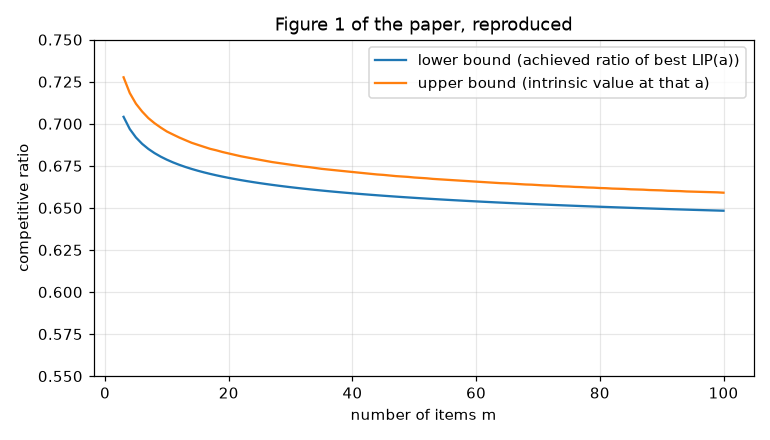
\includegraphics[width=0.8\linewidth]{figures/01_figure1_m_items.png}
\caption{Reproduction of the paper's Figure~1 (its Theorem~3): for each $m=3,\ldots,100$ the LIP
parameter $a$ that maximises the lower bound $\frac{a+b}{a+2mb}\,\underline{\theta}(a)$ is chosen
from $\{0.01,\ldots,20\}$; the lower curve is that bound (an achieved competitive ratio), the
upper curve the intrinsic value $\overline{\theta}(a)$ at the same $a$. The best $a$ grows with
$m$ (about $5.0$ at $m=3$, $9.4$ at $m=100$).}
\label{fig:paper_fig1}
\end{figure}

\subsection{The paper's Theorem~1: the LP upper bound}

\emph{Reminder.} The argument of the paper's Theorem~1 has three steps. (i) Restrict the type space to the
grid $\{j/N\}$: a mechanism only has to serve fewer types, so any upper bound proved on the grid
is valid in general. (ii) On the grid a mechanism is a finite table: for every report profile
$(j,k)$ the shares $p^1_{jk},p^2_{jk}$ of the two items given to agent~1. (iii) Strategy-proofness
and $\alpha$-competitiveness are linear inequalities in the table entries, so the best mechanism
on the grid is a linear program maximising $\alpha$; the paper solves it for $N=50$.

We built the same LP for arbitrary $N$. Its costly part is strategy-proofness: one inequality
per triple (true type, misreport, opponent report), about $8\cdot10^6$ at $N=200$. We keep only
the inequalities between \emph{adjacent} types ($j$ does not want to report $j+1$ and vice
versa), which is $O(N^2)$ and loses nothing: for a fixed opponent report, the utility of a type
$x$ from reporting $j'$, $x\,p^1_{j'}+(1-x)\,p^2_{j'}$, is affine in $x$ with slope
$d_{j'}=p^1_{j'}-p^2_{j'}$. Adding the two adjacent inequalities for $(j,j+1)$ gives
$(x_{j+1}-x_j)(d_{j+1}-d_j)\ge0$, so the slopes are non-decreasing in the report, and with
non-decreasing slopes a type that does not gain from moving one step does not gain from moving
further: for $j<j''$,
\[
U(x_j;j'')=U(x_{j+1};j'')+(x_j-x_{j+1})\,d_{j''}\le U(x_{j+1};j+1)+(x_j-x_{j+1})\,d_{j+1}=U(x_j;j+1)\le U(x_j;j),
\]
by induction on $j''-j$, the sign of $x_j-x_{j+1}$ with $d_{j''}\ge d_{j+1}$, and the adjacent
inequality. This is the single-crossing argument behind Myerson's lemma, and it applies verbatim
in the complementarity model. We verified on grids up to $N=20$ that the full and the reduced LP
agree to $10^{-7}$, and that the mechanism returned by the reduced LP is truthful against every
misreport. With $N=50$ the LP returns $\alpha=0.841225$, the paper's $0.841$.

\paragraph{The bound depends on the grid.} Restricting the type space only removes constraints,
so the LP value is a valid upper bound for every $N$, and the smallest value over $N$ is the one
to quote. It decreases monotonically:
\begin{center}
\begin{tabular}{lcccccccc}
\toprule
$N$ & 40 & 50 & 60 & 80 & 100 & 120 & 150 & 200\\
\midrule
LP value & 0.8429 & 0.8412 & 0.8402 & 0.8388 & 0.8380 & 0.8374 & 0.8368 & 0.8363\\
\bottomrule
\end{tabular}
\end{center}
A least-squares fit $\alpha_N\approx\alpha_\infty+c_1/N+c_2/N^2$ over $N\ge50$ gives
$\alpha_\infty\approx0.8345$ (an extrapolation, not a bound). Only about $N$ of the $(N+1)^2$
competitiveness constraints carry dual weight, and they lie on the edge $x=0$ and on a segment
parallel to the diagonal; eight well-chosen types already certify $0.8734$.
